\documentclass[../main.tex]{subfiles}

\begin{document}
\newpage
\thispagestyle{empty}
\begin{center}
    {
\includegraphics[width=0.5\textwidth]{Imagenes/Logo UMA.jpg}\par}
    \vspace{1cm}
    {\bfseries\LARGE \Facultad \par}
    \vspace{0.5cm}
    {\scshape\Large \Grado \par}
    \vspace{3cm}
    {\scshape\Huge Memoria \par}
    \vspace{1.5cm}
    {\itshape\Large \TituloProyecto \par}
    \vfill
    {\Large Solicitante: \par}
    {\Large \Solicitante  \par}
    \vspace{1cm}
    {\Large Autores: \par}
    {\Large \Autora \par}
    {\Large \Autor \par}
    \vfill
    {\Large \Fecha \par}
\end{center}

\chapter*{Índice de la Memoria:}
\tableof{Memoria}
\newpage
\toftagstart{Memoria}

\section{Objeto}
% En este capítulo de la Memoria se indicrá el objetivo del Proyecto y su justificación.
Este proyecto tiene como objetivo proporcionar información detallada sobre las instalaciones necesarias en una nave industrial con uso de carpintería de madera. Dicha nave se encuentra en Calle Gerald Brenan Nº 37(A), situada en el polígono industrial Guadalhorce de Málaga.

\section{Alcance}
% En este capítulo de la Memoria se indicará el ámbito de aplicación del Proyecto.
El proyecto se centrará en:
\begin{itemize}
    \item Elaboración de planos.
    \item Redacción y diseño de instalaciones de baja tensión, luminaria, saneamiento, fontanería y seguridad contra incendios; asegurando el cumplimiento de la normativa vigente en cada una de estas.
    \item Redacción y diseño de instalaciones de baja tensión, luminaria, saneamiento, fontanería y seguridad contra incendios; asegurando el cumplimiento de la normativa vigente en cada una de estas.
    \item Cálculo del presupuesto.
\end{itemize}

\section{Antecedentes}
% En este capítulo de la Memoria se enumerarán todos aquellos aspectos necesarios para la comprensión de las alternativas estudiadas, y la solución final adoptada.
La parcela de la nave industrial del proyecto se encuentra en el polígono Guadalhorce de Málaga. Esta tiene unas dimensiones de $1400 m^2$, tiene una referencia catastral 8316157UF6681N0001XP. Dicha parcela es de uso industrial y en ella se encuentra la estructura de la nave considerada. \par
\vspace{0.5 cm}
El proyecto se hace por el encargo de \Solicitante, para la asignatura de Oficina Técnica del Grado de Ingeniería Electrónica Industrial de la Universidad de Málaga, y es desarrollado por los alumnos del grado \Autora \ y \Autor.

\section{Normas y referencias}
% En este capítulo de la Memoria se relacionarán sólo los documentos citados en los distintos apartados de la misma.

\subsection{Disposiciones legales y normas aplicadas}
% En este apartado se contemplará el conjunto de disposiciones legales (leyes, reglamentos, ordenanzas, etc.) y las normas de no obligado cumplimiento que se han tenido en cuenta para la realización del Proyecto.
\subsubsection{Instalación de fontanería}
\begin{itemize}
    \item Código Técnico de la Edificación DB-HS4. Suministro de agua.
    \item Reglamento y Normativa Técnica de suministro de agua de EMASA.
    \item UNE 1063:2016 Identificación de canalizaciones según el fluido que transportan.
\end{itemize}

\subsubsection{Instalación de saneamiento}
\begin{itemize}
    \item Documento básico de salubridad. Sección HS5 - Saneamiento.
\end{itemize}

\subsubsection{Instalación de iluminación}
\begin{itemize}
    \item Norma europea sobre la iluminación para interiores-UNE 12464.1 
    \item Código Técnico de la Edificación DB-HE3. Condiciones de las instalaciones de iluminación para el ahorro de energía.
\end{itemize}

\subsubsection{Instalación eléctrica}
\begin{itemize}
    \item Guía técnica de baja tensión
\end{itemize}

\subsection{Bibliografía}
% En este apartado se contemplará el conjunto de libros, revistas u otros textos que el autor considere de interés para justificar las soluciones adoptadas en el Proyecto.
\begin{enumerate}
    \item GUERRERO STRACHAN CARRILLO, J., PÉREZ CARRILLO, B., DE ANDRES DÍAZ, J. R. (2004). Instalaciones eléctricas de baja tensión. Manual básico e imprescindible. España: Ediciones Paraninfo, S.A. 
    \item GUERRERO STRACHAN CARRILLO, J., PÉREZ CARRILLO, B., PLATERO ORTEGA, R. (2004). Diseño e instalaciones de fontanería. Manual básico e imprescindible. España: Ediciones Paraninfo, S.A. 
    \item \textit{Catálogo iluminación profesional Philips | Philips lighting. (n.d.).} Philips Lighting. \\ https://www.lighting.philips.es/soporte/adquisicion/catalogo-iluminacion-profesional-philips    
\end{enumerate}

\subsection{Programas de cálculo}
% En este apartado se contemplará la relación de progrmas, modelos y otras herramientas utilizadas para desarrollar los diversos cálculos del Proyecto.
Para el diseño de las distintas instalaciones y el desarrollo de cierta documentación, se han utilizado los siguientes programas:
\begin{itemize}
    \item DIALux 12.0 del desarrollador DIAL GmbH Lüdenscheid
    \item MATLAB R2022b del desarrollador MathWorks
    \item CYPE 2024 (Castellano). Versión Campus. Uso no profesional - 2024.a del desarrollador CYPE Ingenieros, S.A.
    \item Excel 2023 del desarrollador Microsoft
\end{itemize}

\subsection{Plan de gestión de la calidad aplicado durante la redacción del Proyecto}
% En este apartado se enunciarán los procesos específicos utilizados para asegurar la calidad durante la realización del Proyecto.
\begin{enumerate}
    \item Definición de Requisitos de Calidad:
    \begin{itemize}
        \item Objetivos del Proyecto: Establecimiento claro y preciso de los objetivos del proyecto para garantizar una dirección coherente y alineada.
        \item Expectativas del Cliente: Identificación meticulosa de las necesidades y expectativas del cliente para asegurar la satisfacción del mismo.
    \end{itemize}
    \item Planificación de la Calidad:
    \begin{itemize}
        \item Estandarización: Adopción de estándares de calidad reconocidos en el sector pertinente o la industria específica.
        \item Herramientas y Técnicas: Selección rigurosa de herramientas y técnicas adecuadas para la supervisión y control de la calidad del proyecto.
        \item Criterios de Aceptación: Establecimiento de parámetros y criterios objetivos para determinar la calidad requerida y aceptable.
    \end{itemize}
    \item Implementación de la Calidad:
    \begin{itemize}
        \item Formación y Capacitación: Provisión de formación especializada y capacitación continua al equipo de proyecto en relación con los estándares y procesos de calidad.
        \item Revisión Continua: Ejecución de revisiones periódicas y sistemáticas para asegurar la adherencia a los estándares de calidad preestablecidos.
        \item Control de Documentación: Supervisión constante para garantizar que toda la documentación asociada al proyecto sea precisa, actualizada y cumpla con los estándares de calidad.
    \end{itemize}
    \item Monitoreo y Control de la Calidad:
    \begin{itemize}
        \item Auditorías de Calidad: Realización de auditorías regulares para evaluar el cumplimiento de los estándares y procedimientos de calidad.
        \item Medición y Análisis: Aplicación de métricas y KPIs (Indicadores Clave de Desempeño) para evaluar y monitorear el progreso y desempeño del proyecto.
        \item Acciones Correctivas: Implementación oportuna de acciones correctivas en respuesta a desviaciones o discrepancias identificadas en relación con la calidad.
    \end{itemize}
    \item Mejora Continua:
    \begin{itemize}
        \item Retroalimentación: Recolección sistemática de retroalimentación tanto del cliente como del equipo de proyecto para identificar áreas de mejora.
        \item Análisis de Causa Raíz: Aplicación de técnicas avanzadas, como el análisis de causa raíz, para identificar y abordar las causas subyacentes de los problemas de calidad.
        \item Optimización de Procesos: Revisión y ajuste continuo de procesos y procedimientos con el objetivo de mejorar la eficiencia y eficacia en la gestión de calidad.
    \end{itemize}
    \item Comunicación:
    \begin{itemize}
        \item Comunicación Efectiva: Establecimiento de canales de comunicación claros y efectivos con todas las partes interesadas para asegurar la alineación y entendimiento mutuo respecto a los estándares y objetivos de calidad.
        \item Feedback: Fomento y facilitación de la retroalimentación entre todas las partes involucradas para promover la mejora continua y la adaptabilidad en el proceso de gestión de calidad.
    \end{itemize}
\end{enumerate}
En conclusión, la implementación efectiva del presente plan de gestión de calidad durante la redacción del proyecto garantizará la consecución de los estándares de calidad establecidos, así como la satisfacción de los requisitos y expectativas del cliente y demás partes interesadas.

\subsection{Otras referencias}
% En este apartado se incluirán aquellas referencias que, no estando relacionadas en los apartados anteriores, se consideren de interés para la comprensión y materialización del Proyecto.
\begin{itemize}
    \item Bruno. (2021, August 16). \textit{Procedimiento de cálculo de tuberías para una instalación de fontanería.} IngenierosIndustriales.com. https://www.ingenierosindustriales.com/procedimiento-de-calculo-de-tuberias-para-una-instalacion-de-fontaneria/
    \item \textit{Instalaciones. Normativa nacional. (n.d.).} \\ http://normativaconstruccion.cype.info/Instalaciones.html\#gsc.tab=0
    \item Luxes. (2022, October 27). \textit{Normativa de iluminación en espacios de trabajo.} Luxes. \\ https://luxes.es/normativa-de-iluminacion-en-espacios-de-trabajo/
    \item \textit{Instalaciones de Fontanería - Construmatica.} (n.d.). \\ https://www.construmatica.com/construpedia/Instalaciones\_de\_Fontaner\%C3\%ADa
\end{itemize}
\section{Definiciones y abreviaturas}
% En este capitulo de la Memoria se relacionarán todas las definiciones, abreviaturas, etc. que se han utilizado y su significado.
\subsection{Instalación de fontanería}
\begin{table}[H]
    \centering
    \begin{tabular}{l|l}
         Abreviatura & Significado \\ \hline
         EMASA & Empresa Municipal Aguas de Málaga \\ \hline
         ACS & Agua Caliente Sanitaria \\ \hline
         Q & Caudal \\ \hline
         K & Coeficiente de simultaneidad \\ \hline
         n & Número de aparatos en la red \\  \hline
         v & Velocidad del agua \\ \hline
         D & Diámetro \\ \hline
         PVC & Policloruro de vinilo \\ \hline
         $\rho$ & Densidad del fluido \\ \hline
         $\mu$ & Viscosidad dinámica del fluido \\ \hline
         Re & Número de Reynolds \\ \hline
         e & Rugosidad de la tubería \\ \hline
         hf & Pérdida de carga debida a la fricción \\ \hline
         f & Factor de fricción de Darcy \\ \hline
         L & Longitud \\ \hline
         g & Aceleración de la gravedad \\ \hline
         mca & Metros Columna de Agua \\ \hline
         V & Volúmen \\ \hline
         t & Tiempo \\ \hline
         Pb & Presión mínima de arranque \\ \hline
         Ha & Altura geométrica de aspiración \\ \hline
         Hg & Altura geométrica \\ \hline
         Pc & Pérdida de carga del circuito \\ \hline
         Pr & Presión residual en el grifo, llave o fluxor \\ \hline
         Vn & Volumen útil del depósito de membrana \\ \hline
         Va & Volumen mínimo de agua \\ \hline
         Pa & Presión absoluta máxima
    \end{tabular}
    \caption{Abreviaturas y definiciones de fontanería.}
\end{table}

\subsection{Instalación de saneamiento}
\begin{table}[H]
    \centering
    \begin{tabular}{l|l}
    Abreviatura & Significado \\ \hline
    EMASA & Empresa Municipal Aguas de Málaga \\ \hline
    i & Intensidad pluviometrica [mm/h] \\ \hline
    f & factor de correción \\ \hline
    Msph & Máxima superficie en proyección horizontal \\ \hline
    PVC & Policloruro de vinilo \\ \hline
    Sph & Superficie en proyección horizontal \\ \hline
    UD & Unidades de desagüe \\ \hline
    \end{tabular}
    \caption{Abreviaturas y definiciones de saneamiento.}
\end{table}



\subsection{Instalación de iluminación}
\begin{table}[H]
    \centering
    \begin{tabular}{l | l}
         Abreviatura & Significado \\ \hline
         UGR & Índice de deslumbramiento unificado \\ \hline
         VEII & Valor de eficiencia energética de la instalación \\ \hline
         Ra & Índice de rendimiento cromático \\ \hline
         Uo & Uniformidad de iluminancia \\ \hline
         Em & Iluminancia media \\ \hline
         P & Potencia \\ \hline
         $\phi$ & Flujo luminoso \\ \hline
         Lx & Unidad de medición del nivel de iluminación \\ \hline
         Lm & Unidad de medición del flujo luminoso \\ \hline
         W & Vatios
    \end{tabular}
    \caption{Abreviaturas y definiciones de iluminación.}
\end{table}

\subsection{Instalación eléctrica}

\begin{table}[H]
    \centering
    \begin{tabular}{l | l}
         Abreviatura & Significado \\ \hline
         V & Voltios \\ \hline
         I & Intensidad \\ \hline
         A & Amperios \\ \hline
         $\rho$ & Resistividad \\ \hline
         W & Vatios \\ \hline
         P & Potencia \\ \hline
    \end{tabular}
    \caption{Abreviaturas y definiciones de la instalación eléctrica}
\end{table}


\section{Requisitos de diseño}
% En este capítulo de la Memoria se describirán las bases y datos de partida establecidos.

\subsubsection{Requisitos de las instalaciones}
En el presente taller se requiere que todas las instalaciones que lo conforman estén diseñadas conforme a la norma actual. \par
\vspace{0.5 cm}
La instalación de baja tensión será dimensionada para poder suministrar la potencia necesaria a las máquinas del taller, así como la iluminación y las tomas de corriente que se encuentran en la nave. \par
\vspace{0.5 cm}
Para asegurar la presión mínima de agua en la nave, se cuenta con un grupo de presión que actuará en caso de que la presión de suministro por parte de EMASA sea menor que la contratada de forma excepcional. \par
\vspace{0.5 cm}
Se diseñará también una instalación contra incendios que incluya los equipos extintores necesarios, sistema de alarma, iluminación de emergencia y ruta de evacuación. Además de la instalación de saneamiento para aguas residuales y aguas pluviales. \par

\subsubsection{Dimensiones del espacio}
Se cuenta con la estructura de una nave localizada en el Polígono Industrial Guadalhorce de Málaga. 

\section{Descripción del proyecto}
\subsubsection{Proceso productivo}
La materia prima se almacenará en almacén. Este está equipado con una entrada directa dimensionada para permitir la entrada y salida de carretillas elevadoras, también cuenta con una entrada hacia la planta de producción igual dimensionada. Una vez la materia prima se encuentre en la planta de producción podrán dirigirse a las maquinas para su corte y procesado. Si fuese necesario se trasladarían posteriormente a las maquinas CNC donde se realizarían los cortes más precisos. Finalmente se haría uso de las maquinas manuales que se encuentran en los bancos de trabajo para ultimar detalles del producto. Una vez se obtenga el producto finalizado, este pasará al almacén. \par
\vspace{0.5 cm}
Cabe destacar que la planta de producción cuenta con una aspiradora que permitirá la aspiración automática de virutas para desclasificar la nave como de riesgo de explosión, según se indica en el reglamento electrotécnico de baja tensión. \par
\vspace{0.5 cm}
Además se contará con espacio suficiente, tanto en el almacén como en la planta de producción, entre máquinas para una fácil manipulación y transporte tanto de la materia prima como de los productos acabados. 

\subsubsection{Maquinaria empleada en el taller}
La maquinaria que se ha considerado necesaria para dicha carpintería incluirá aquella para 
\begin{itemize}
    \item Combinada de 5 operaciones \\
    Número de unidades: 2
    \begin{figure}[H]
        \centering
        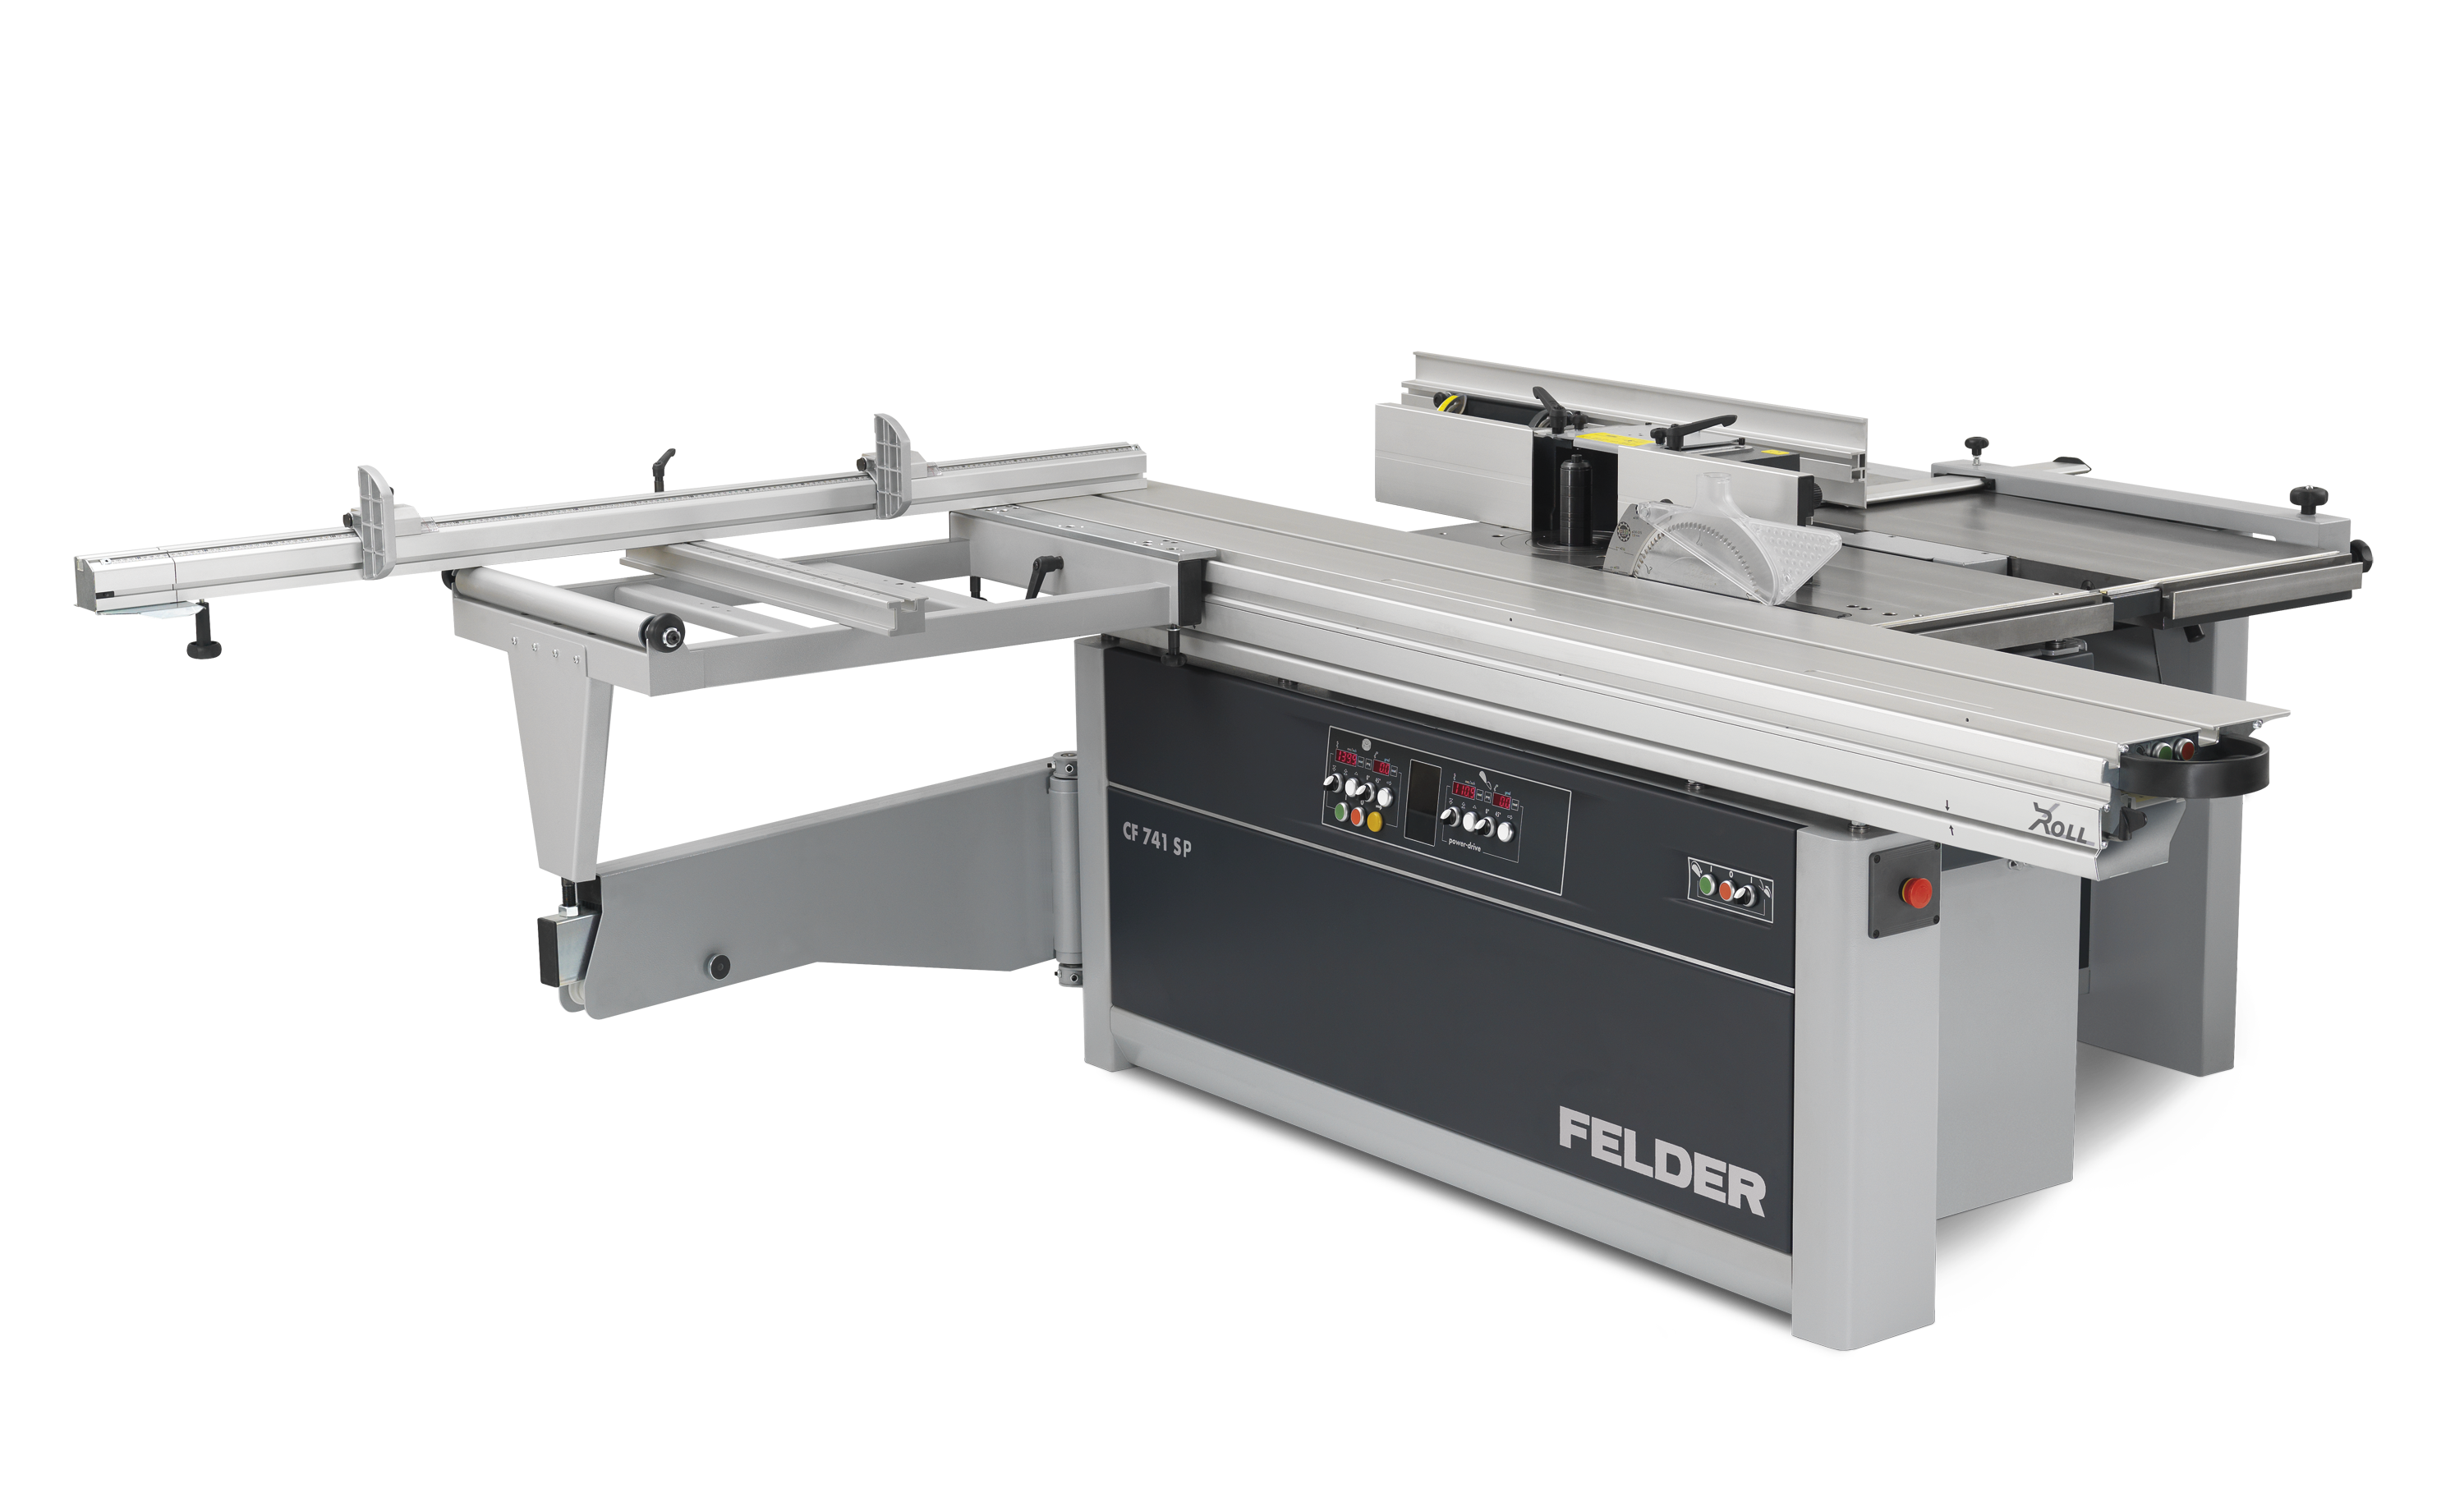
\includegraphics[width=0.5\linewidth]{Imagenes/Combinada5Operaciones.png}
        \caption{Felder CF 741 S Profesional.}
    \end{figure}
    
    \item CNC Grande \\
    Número de unidades: 1
    \begin{figure}[H]
        \centering
        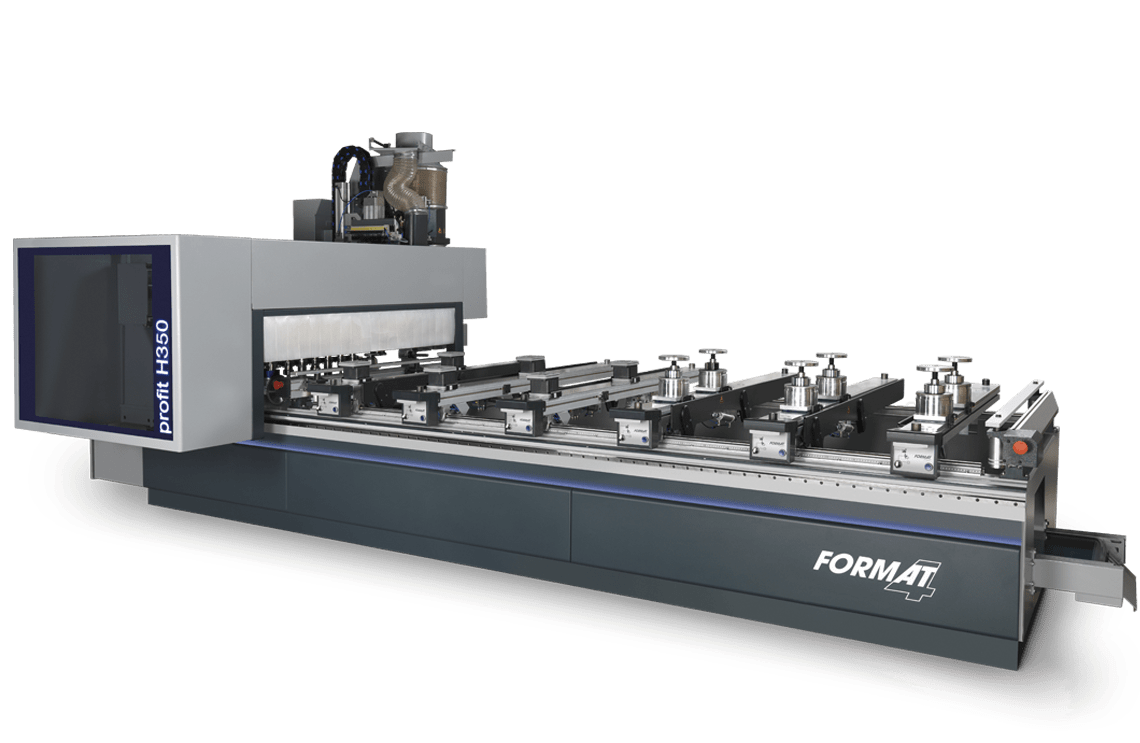
\includegraphics[width=0.5\linewidth]{Imagenes/CNCGrande.png}
        \caption{Format Profit H350 - 16.30.}
    \end{figure}

    \item CNC Pequeña \\
    Número de unidades: 2
    \begin{figure}[H]
        \centering
        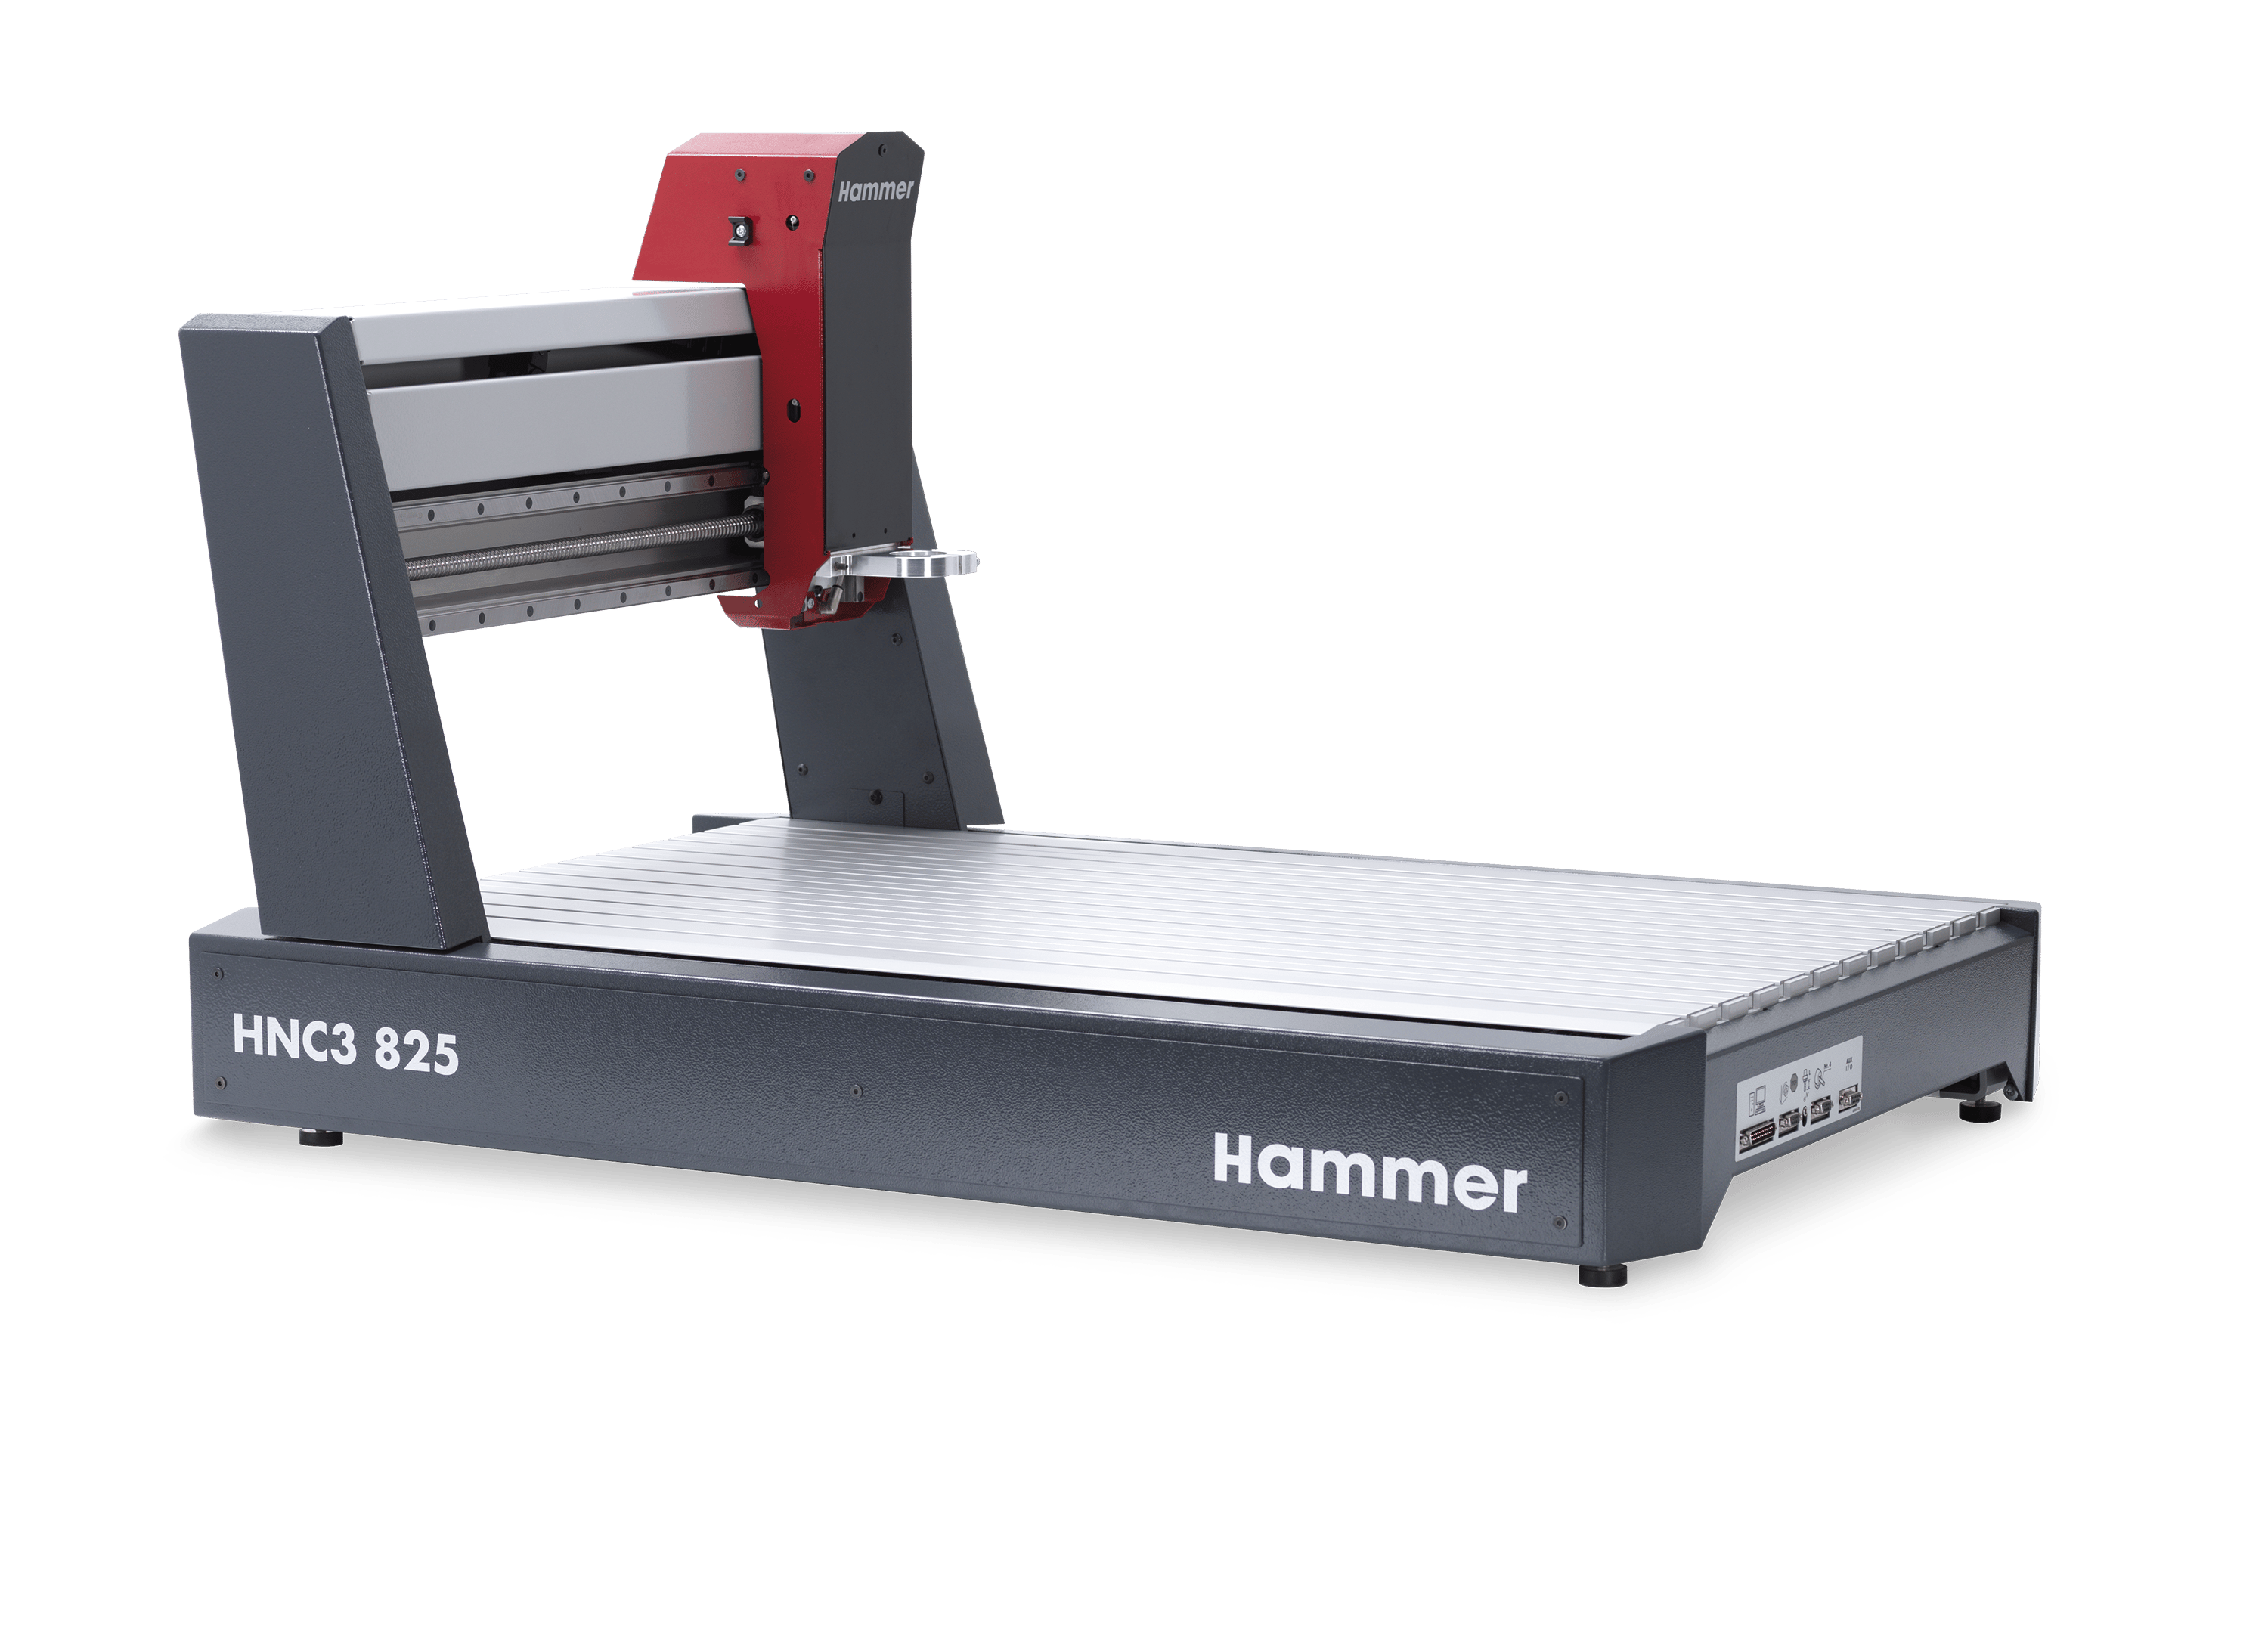
\includegraphics[width=0.5\linewidth]{Imagenes/CNCPequena.png}
        \caption{Hammer HNC3 825 Perform.}
    \end{figure}

    \item Lijadora \\
    Número de unidades: 1
    \begin{figure}[H]
        \centering
        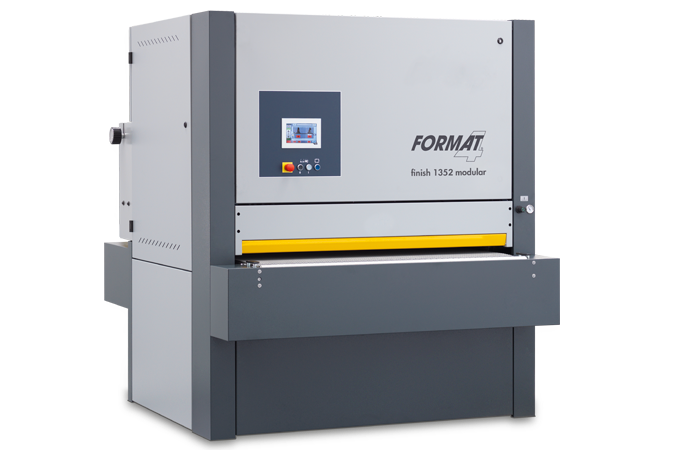
\includegraphics[width=0.5\linewidth]{Imagenes/Lijadora.png}
        \caption{Format Findustry 1352.}
    \end{figure}

    \item Seccionadora Vertical \\
    Número de unidades: 1
    \begin{figure}[H]
        \centering
        \includegraphics[width=0.5\linewidth]{Imagenes/SeccionadoraVertical.png}
        \caption{Enter Caption}
        \label{fig:enter-label}
    \end{figure}

    \item Briquetadora \\
    Número de unidades: 1
    \begin{figure}[H]
        \centering
        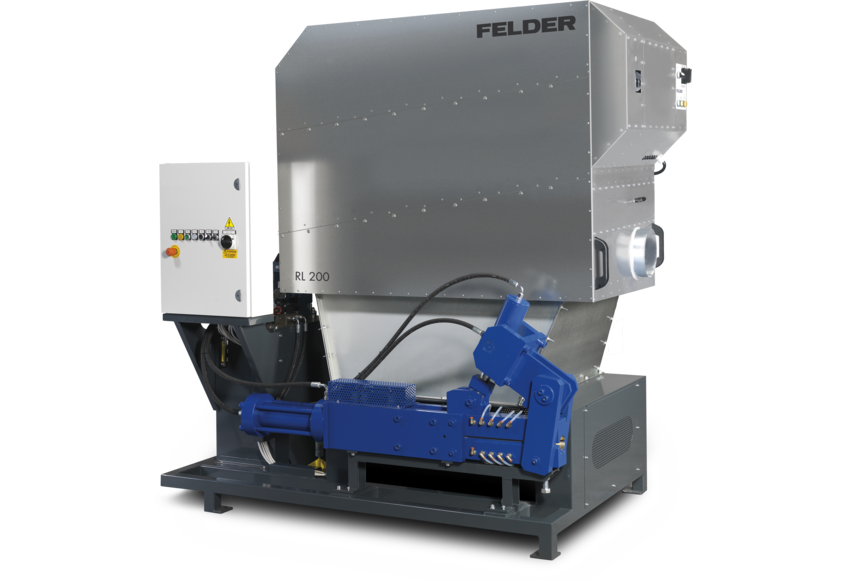
\includegraphics[width=0.5\linewidth]{Imagenes/Briquetadora.png}
        \caption{Felder FBP 70.}
    \end{figure}
    
\end{itemize}

Además se cuenta con dos mesas de trabajo que contará con maquinaria manual para el tratado en detalle de la madera. Dichos bancos son los siguientes:
\begin{figure}[H]
    \centering
    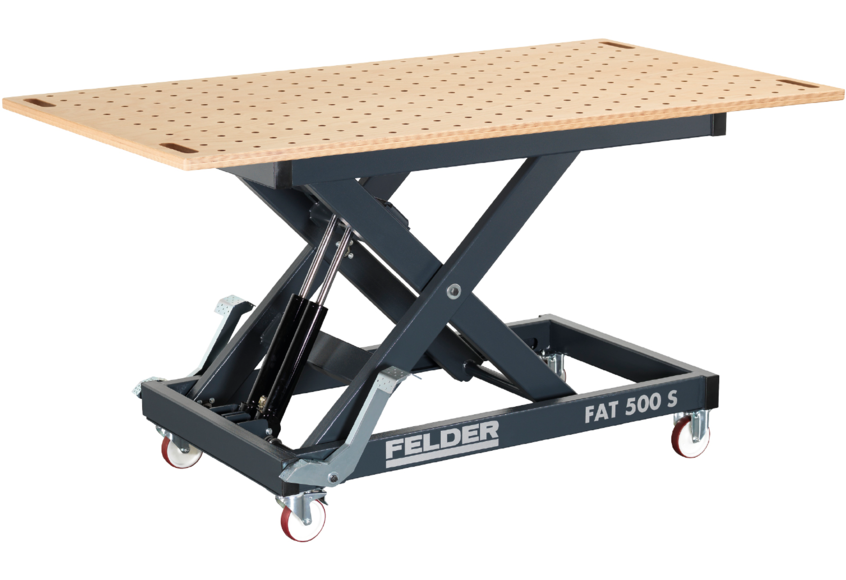
\includegraphics[width=0.5\linewidth]{Imagenes/MesaTrabajo.png}
    \caption{Felder FAT 500 S.}
\end{figure}

Para asegurar se contará con el siguiente grupo de aspiración:
\begin{figure}[H]
    \centering
    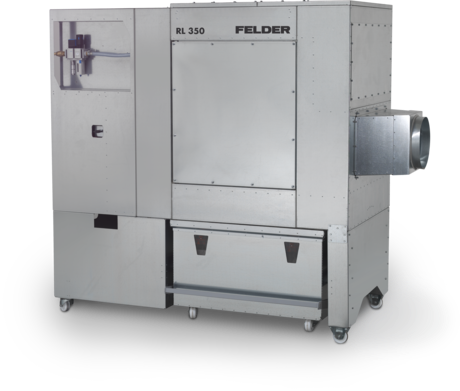
\includegraphics[width=0.5\linewidth]{Imagenes/GrupoAspiracion.png}
    \caption{Felder RL350.}
\end{figure}
\section{Análisis de soluciones}
% En este capítulo de la Memoria se indicarán las distintas alternativas estudiadas, qué caminos se han seguido para llegar a ellas, ventajas e inconvenientes de cada una y cuál es la solución finalmente elegida y su justificación.
\subsection{Instalación de fontanería}
En el diseño de la instalación de suministro de agua para la nave se tiene en cuenta la normativa vigente para ello. Considerando lo establecido por la compañía suministradora, EMASA, y el Código Técnico de la Edificación. \par
\vspace{0.5 cm}
La acometida será de PVC y será dimensionada según la demanda del edificio. La tubería de esta estará unida a la llave de corte general del edifico y a la caja de contadores, y estará situada en la parte exterior del este. Las tuberías de la instalación interior discurrirán por el exterior de los tabiques a una altura considerable y cercana al techo cuando sea posible. Estas tuberías serán de acero galvanizado y seguirán la norma UNE 1063 de identificación de canalizaciones según el fluido que transportan. \par
\vspace{0.5 cm}
Teniendo en cuenta los aparatos que se encuentra en la nave, su caudal mínimo instantáneo tanto de agua fría como de ACS y las pérdidas de carga en el circuito, se elegirá un diámetro nominal para las tuberías de cada tramo asegurando que la velocidad del agua se mantiene dentro del rango de 0,50 y 2,00 m/s para tuberías metálicas. \par
\vspace{0.5 cm}
Cabe destacar que la presión suministrada en la acometida por EMASA es de $1,94 bar$ y que puede oscilar un $\pm 20 \%$. Se debe asegurar una presión mínima en el punto de consumo, que según lo establecido en el CTE HS4, será de $10 mca$ en el caso de grifos comunes y de $15 mca$ en el caso de calentadores. Si en el caso más desfavorable, la presión que se alcanza en el punto de consumo fuese menor que la establecida, se deberá instalar un grupo de presión auxiliar. Además, esta presión nunca será mayor de $500 kPa$. \par

\subsection{Instalación de saneamiento}

En el diseño de la instalación de saneamiento, se ha considerado el documento básico de Salubridad en su sección HS 5, denominada, Evacuación de aguas. 

Además se ha contactado con la empresa EMASA, para conocer en detalle el tipo de saneamiento existente en la calle Gerald Brenand. Ante la respuesta de esta, se decide realizar dos instalaciones: Una de saneamiento fluvial y otra de saneamiento residual. 

La instalación de saneamiento fluvial, está destinada a la evacuación de la lluvia en todas las superficies exteriores de la nave, tanto cubiertas como aparcamiento. La instalación se ocupa tanto de los canalones, bajantes y colectores en PVC hasta un pozo general y su acometida.

La instalación de saneamiento residual está destinada a la evacuación de los fluidos generados en los aseos y vestuarios. La instalación se ocupa tanto de derivaciones individuales, bajantes y colectores, en PVC, hasta otro pozo y su acometida.

\subsection{Instalación de iluminación}
Para el cálculo de la iluminación, se seguirá la normativa mencionada anteriormente en la presente memoria. Dicha normativa establece los parámetros de iluminación que se deben cumplir en función del uso de la estancia.

\begin{table}[H]
    \centering
    \begin{tabular}{c | c | c | c | c | c | c }
         Estancia & Em & UGR & Uo  & Ra & VEEI & Pmáx \\ \hline
         Planta de Producción & 500 & 19 & 0,6 & 80 & 5,0 & 25 \\
         Baños & 200 & 25 & 0,4 & 80 & 4,0 & 10 \\
         Baño Minusválidos & 200 & 25 & 0,4 & 80 & 4,0 & 10 \\
         Zona Exposición & 300 & 22 & 0,4 & 80 & 4,0 & 10 \\
         Oficina & 500 & 19 & 0,6 & 80 & 3,0 & 10 \\
         Almacén & 100 & 25 & 0,4 & 60 & 4,0 & 10 \\
         Vestuarios & 200 & 25 & 0,4 & 80 & 4,0 & 10 \\
         Zona Descanso& 100 & 22 & 0,4 & 80 & 4,0 & 10 \\
    \end{tabular}
    \caption{Parámetros de iluminación de las estancias en la nave.}
\end{table}

Para un correcto cumplimiento de la norma, los resultados luminotécnicos obtenidos deberán cumplir lo siguiente:

\begin{itemize}
    \item La iluminancia media (Em) tendrá que ser mayor a la indicada en la norma.
    \item El índice de deslumbramiento unificado (UGR) máximo calculado deberá ser menor que el indicado por la normativa para el tipo de actividad que se realiza en la estancia.
    \item La uniformidad de la iluminancia (Uo) obtenida debe ser mayor a la dispuesta en la normativa.
    \item La reproducción cromática (Ra) mínima calculada deberá ser mayor que la indicada por la norma para dicha estancia.
    \item El valor de eficiencia energética de la instalación (VEII) no superará el valor límite establecido en la Tabla 3.1-HE3.
    \item La potencia total (Pmáx) de lámparas y equipos auxiliares por superficie iluminada no superará el valor máximo establecido en la Tabla 3.2-HE3.
\end{itemize}

Respecto a los parámetros de cálculo utilizados, consideramos un factor de mantenimiento o factor de degradación global de 0,8, y unos grado de reflexión de techo, paredes y suelo de 70.0 \% 50.0 \% y 20.0 \% respectivamente. \par
\vspace{0.5 cm}
El conjunto de luminarias seleccionadas deberán cumplir los parámetros detallados en la tabla anterior. Su elección se ha llevado a cabo con la finalidad de instalar la mínima potencia posible que cumpla con la norma previamente expuesta.\par

\subsection{Instalación eléctrica}

En el diseño de la instalación electrica, se ha empleado la guía técnica de baja tensión.

Se ha empleado para obtener las secciones mínimas, el aislante y el método de instalación conveniente en cada lugar de la nave taller. 

Se ha realizado también en la instalación eléctrica, su acometida y el estudio de protecciones de esta.

\section{Resultados finales}
% En este capítulo de la Memoria se describirá el producto, obra, instalación, servicio o software (soporte lógico) según la solución elegida, indicando cuáles son sus características definitorias y haciendo referencia a los planos y otros elementos del Proyecto que lo definen.

\subsection{Instalación de fontanería}
\subsubsection{Acometida}
Se dispone una acometida de tubo de PVC de 25 mm de diámetro que irá conectado a la red pública de abastecimiento hasta el contador general empotrado en el muro exterior de la nave. Esta acometida tendrá un caudal de $0,85 dm^3/s$ a una velocidad del agua de $1,7 m/s$.

\subsubsection{Instalación general}
Según lo indicado en el DB HS-4 la instalación general debe contener lo siguiente:
\begin{itemize}
    \item Llave de corte general. \\
    Servirá para interrumpir el suministro al edificio y estará situada en el interior del armario de contador general.
    \item Filtro de la instalación general. \\
    Retendrá los residuos del agua que puedan dar lugar a corrosiones en las canalizaciones metálicas. Este será de tipo Y con un umbral de filtrado de entre $25$ y $50 \mu m$, con malla de acero inoxidable y baño de plata, para evitar la formación de bacterias y autolimpiable.
    \item Armario o arqueta del contador general. \\
    Este contendrá, dispuestos en este orden, la llave de corte general, un filtro de la instalación general, el contador, una llave, grifo o racor de prueba, una válvula de retención y una llave de salida. \\
    Según lo establecido en los reglamentos, normas y documentación técnica para el abastecimiento de EMASA, para un diámetro de acometida de 25 mm, el armario de contadores deberá tener unas medidas mínimas de 1000 mm de largo, 320 mm de ancho y 500 mm de alto. Además las marcas y/o modelos autorizados de este son HIMEL, PLA 2540 EMASA.
    \item Tubo de alimentación. \\
    Discurrirá enterrado en el suelo y se tendrá acceso a sus extremos y cambios de dirección para su inspección y control de fugas.
    \item Distribuidor principal. \\
    Al igual que el tubo de alimentación, irá enterrado en el suelo y se dispondrá de registros para su inspección y control de fugas. Se dispondrá de llaves de corte en todas las derivaciones, de forma que en caso de avería en cualquier punto no deba interrumpirse todo el suministro.
\end{itemize}

\subsubsection{Instalación de agua fría}
Esta suministrará el agua necesaria a los diferentes puntos de consumo en la nave, y está compuesta por las tuberías, codos y llaves de paso. \par
\vspace{0.5 cm}
Las tuberías tienen un trazado simple por el exterior de los muros. Estas se agarrarán al mismo mediante abrazaderas. Además no discurrirán por zonas susceptibles a remodelación. Estas cuentan también con llaves de corte para que en caso de avería se pueda cortar el suministro en dicho tramo sin parar el suministro en el resto de la instalación. \par
\vspace{0.5 cm}
Los detalles de los tramos que conforman la instalación de agua fría se muestran en la siguiente tabla:
\begin{table}[H]
    \centering
    \begin{tabular}{c | c | c | c | c | c | c | c | c}
         Tramo & $Q [l/s]$ & $K$ & $Q_c [l/s]$ & $v [m/s]$ & $D_{min} [mm]$ & $D_{int} [mm]$ & $D_{ext} [mm]$ & $v_{real} [m/s]$ \\ \hline
         1 & 3,4 & 0,20 & 0,68 & 1,7 & 22,5676 & 25 & 27 & 1,3853 \\
         2 & 0,60 & 0,4472 & 0,2683 & 1,7 & 14,1763 & 16 & 18 & 1,3344\\
         3 & 0,20 & 1 & 0,20 & 1,7 & 12,239 & 16 & 18 & 0,9947\\
         4 & 0,60 & 0,4472 & 0,2683 & 1,7 & 14,1763 & 16 & 18 & 1,3344 \\
         5 & 1 & 0,4472 & 0,4472 & 1,7 & 18,3016 & 20 & 22 & 1,4235 \\
         6 & 1 & 0,4472 & 0,4472 & 1,7 & 18,3016 & 20 & 22 & 1,4235\\
    \end{tabular}
    \caption{Resultados de los tramos de agua fría.}
\end{table}

\subsubsection{Instalación de agua caliente sanitaria (ACS)}
Las tuberías de agua caliente sanitaria tendrán un trazado similar al de las tuberías de agua fría. Esta será suministrada y almacenada por un termo eléctrico conectado a la instalación de agua fría y a la misma. Los detalles de los tramos de ACS se detallan en la siguiente tabla:

\begin{table}[H]
    \centering
    \begin{tabular}{c | c | c | c | c | c | c | c | c}
         Tramo & $Q [l/s]$ & $K$ & $Q_c [l/s]$ & $v [m/s]$ & $D_{min} [mm]$ & $D_{int} [mm]$ & $D_{ext} [mm]$ & $v_{real} [m/s]$ \\ \hline
         7 & 1,3850 & 0,25 & 0,3463 & 1,7 & 16,1037 & 20 & 22 & 1,1023\\
         8 & 0,3250 & 0,50 & 0,1625 & 1,7 & 11,0321 & 16 & 18 & 0,8082\\
         9 & 0,53 & 0,4472 & 0,2370 & 1,7 & 13,3237 & 16 & 18 & 1,1787\\
         10 & 0,53 & 0,4472 & 0,2370 & 1,7 & 13,3237 & 16 & 18 & 1,1787\\
    \end{tabular}
    \caption{Resultados de los tramos de ACS.}
\end{table}

El termo eléctrico de agua elegido para el abastecimiento de ACS para la nave es el Bosch Termo eléctrico Tronic 6000T con una capacidad de 150 litros.

\subsubsection{Grupo de presión}
Teniendo una presión de suministro por parte de EMASA en la acometida de $1,94 bar = 19,7830 mca$ y oscilando esta un $\pm 20 \%$, en el caso más desfavorable, la presión final en el punto de consumo es menor a la requerida por el CTE DB-HS4, por lo que es necesario un grupo de presión auxiliar. Dicha instalación dispondrá de:
\begin{itemize}
    \item Depósito auxiliar de alimentación de $1000 l$.
    \item 2 Bombas de presión de agua STERWINGS de $900 W$ de potencia con calderín de $24 l$.
    \item Depósito de presión Imera de $12 l$
\end{itemize}

\subsection{Instalación de saneamiento}

La instalación de saneamiento se divide en 2 partes. La instalación pluvial

\subsubsection{Saneamiento pluvial}

Se ha designado la instalación de un canalón a cada lado de la cubierta, de PVC, de 25 $ mm^2$ y una inclinación del 1\%. Dicho canalón puede evacuar el agua caída con una intensidad pluviométrica de 110 mm/h de un total de 431.81 $ m^2$. Superior a la superficie en cubierta horizontal de la mitad de la cubierta, que es un total de 420 $m^2$.

Para la evacuación del agua caída en los canalones, se decide poner 3 bajantes por cada canalón, 6 en total.

Con una sola bajante en cada canalón podría evacuar el agua, pero se ha decidido aumentar su número a 6. Debido a que en una zona industrial, con elevado polvo en suspensión, podría obstruir una bajante. 

Cada bajante cumple una superficie horizontal de 110 mm/h. La bajante propuesta es una de PVC 75 mm, a pie de estas se instala un bote no sifónico.

Los colectores se encargan de transportar el agua de forma horizontal, desde una bajante o un sumidero hasta un bote (sifónico o no) o hasta el pozo general.

Todos los colectores son enterrados y por tanto, con una pendiente mínima del 2\%.

Cada bajante, conectada a un bote no sifonico, tiene un colector de salida de 90 mm, con una pendiente del 2\%.

Los colectores se unen, en botes no sifónicos. Se ha realizado de la siguiente forma:

\begin{itemize}
    \item 2 Colectores de 90 mm, provenientes de las bajantes a un bote no sifónico, cuya salida es un colector de 110 mm y una inclinación del 2\%
    \item 2 Colectores de 90 mm, provenientes de las bajantes y el colector anterior de 110 mm a un bote no sifónico, cuya salida es otro colector de 125 mm e inclinación 3\%
    \item 2 Colectores de 90 mm, provenientes de las bajantes y el colector anterior de 125 mm a un bote no sifónico, cuya salida es otro colector de 160 mm e inclinación 3\%
\end{itemize}

Este último acaba en el pozo general.

Para los sumideros en el aparcamiento, se ha dividido este en 4 zonas:

\begin{table}[H]
    \centering
    \begin{tabular}{c|c}
         Nombre & Superficie [$m^2$] \\ \hline
         Zona 1 & 142.5 \\
         Zona 2 & 123.5\\
         Zona 3 & 130\\
         Zona 4 & 150\\
    \end{tabular}
    \caption{Subzonas del aparcamiento}
\end{table}

A cada sumidero, instalado en el centro de cada zona, se instala un colector enterrado de 90 mm y 2\% de pendiente.

El colector de la zona 3 y de la zona 4, son conectados a un bote, no sifónico, sale un colector de 110 mm de diámetro y una pendiente del 2\%

El colector de la zona 1, el de la zona 2 y el colector saliente del anterior bote, se unen en otro bote, del que sale un tercer colector de 125 mm de diámetro y 3\% de pendiente que acaba en el pozo general de la instalación.

Del pozo general, sale un último colector, dicho colector es de 200 mm de diámetro y una pendiente del 2\%.

\subsubsection{Saneamiento Residual}

Se decide la instalación de sifones individuales en lugar de un bote sifónico.

Las derivaciones individuales quedan reflejadas en la siguiente tabla:

\begin{table}[H]
    \centering
    \begin{tabular}{c|c}
    Zona & UD total \\ \hline
    Baño masculino y femenino & 24 \\
    Baño de minusválidos & 7 \\
    Vestuarios & 16 \\
    \end{tabular}
    \caption{Derivaciones individuales}
\end{table}

Debido a que los vestuarios están en la entreplanta, se instala una bajante de 63 mm de diámetro, con capacidad máxima de 19 UD.

Con el empleo de los colectores individuales se transporta los desechos residuales hasta otro pozo, antes de la acometida. 

Los desechos de ambos baños son evacuados con colectores de 63 mm de diámetros con un 4\% de pendiente.

Los desechos del baño de minusválidos son evacuados con un colector horizontal de diámetro 50 mm y pendiente del 2\%.

Los 3 colectores anteriormente mencionados se unen en uno, de diámetro 90 mm y con una pendiente del 2\%.

A este colector se le añade el colector proveniente de la bajante del vestuario. Acabando así con un colector de diámetro 90 mm y pendiente del 2\%. Este colector acaba en otro pozo general del edificio, donde de ahí, evacua con otro colector del mismo diámetor y misma pendiente.

\subsection{Instalación de iluminación}
\subsubsection{Resultados obtenidos en DIALux Evo}
En la siguiente tabla se muestran los resultados de los parámetros luminotécnicos obtenidos en DIALux para cada estancia, cumpliendo con los requisitos de estos mencionados anteriormente en la presente memoria.

\begin{table}[H]
    \centering
    \begin{tabular}{c | c | c | c | c | c}
         Estancia & Em & Uo & UGR & Pmáx & VEEI \\ \hline
         Planta de Producción & 522 & 0,48 & 17 & 3.225,6 & 1,00\\ 
         Baños & 227 & 0,45 & 18 & 42,0 & 1,79 \\ 
         Baño minusválidos & 276 & 0,53 & 18 & 42,0 & 2,23\\ 
         Zona Exposición & 347 & 0,46 & 22 & 235,2 & 1,57 \\ 
         Oficina & 592 & 0,64 & 19 & 73,2 & 1,24 \\ 
         Almacén & 117 & 0,52 & 16 & 196,0 & 1,50 \\ 
         Vestuarios & 290 & 0,45 & 20 & 85,5 & 1,45 \\ 
         Zona Descanso & 116 & 0,40 & 21 & 57,0 & 1,19
    \end{tabular}
    \caption{Resultados instalación de iluminación.}
\end{table}

Se obtienen también la lista de luminarias a utilizar. Dichas luminarias se han seleccionado del catálogo para profesionales de Philips. En caso de sustitución de dichas luminarias por otras, estas deberán ser de características similares, para asegurar el cumplimiento de una correcta iluminación en la nave. Dichas luminarias empleadas son las siguientes:

\begin{figure}[H]
    \centering
    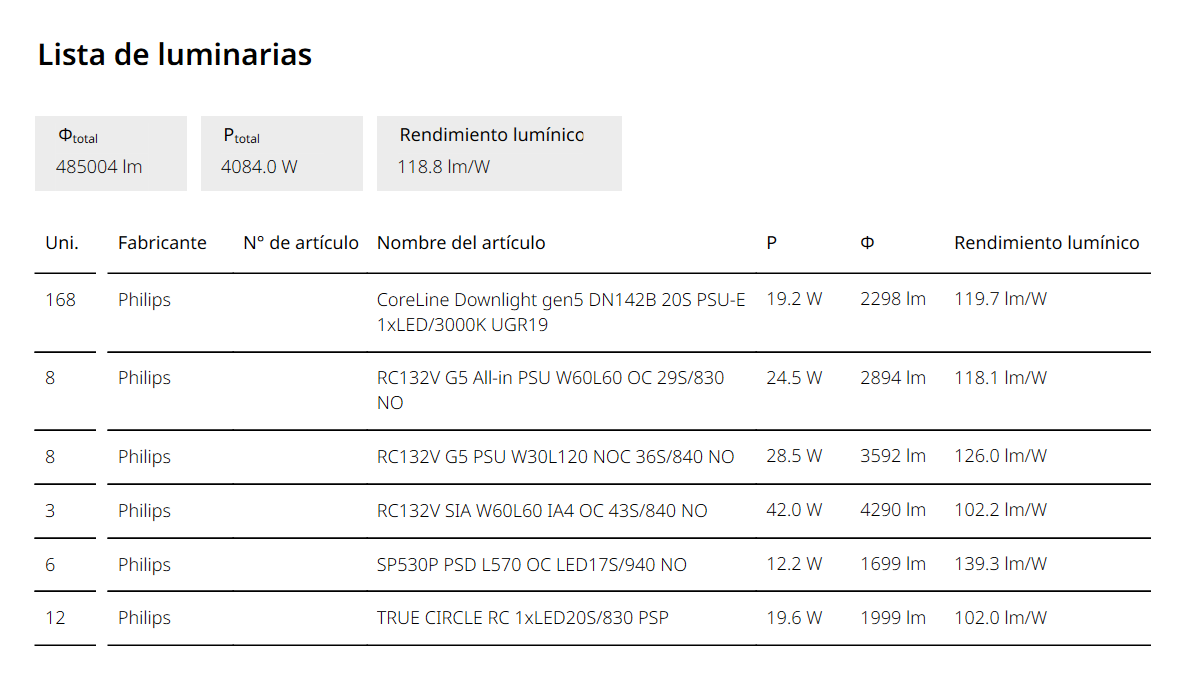
\includegraphics[width=0.75\linewidth]{Imagenes/Lista de luminarias.png}
    \caption{Luminaria empleada en la nave.}
\end{figure}

\subsubsection{Potencia Total Instalada}
La potencia total instalada para la iluminación será de 4.084 W aproximadamente. En la siguiente tabla se detalla la potencia para cada una de las estancias de la nave. Para los baños y vestuarios se indica la potencia de uno de ellos (femenino o masculino), teniendo en cuenta que ambos son idénticos.

\begin{table}[H]
    \centering
    \begin{tabular}{c | c }
         Estancia & Ptotal [W] \\ \hline
         Planta de Producción & 3.225,6 \\ 
         Baños & 42,0 \\ 
         Baño minusválidos & 42,0 \\ 
         Zona Exposición & 235,2 \\ 
         Oficina & 73,2 \\ 
         Almacén & 196,0 \\ 
         Vestuarios & 85,5 \\ 
         Zona Descanso & 57,0 \\ 
         Total Nave & 4.084
    \end{tabular}
    \caption{Potencia instalada para iluminación.}
\end{table}


\subsubsection{Sistema de control de luminarias}
Para el sistema de control de encendido/apagado de las luminarias se contará con al menos un sistema manual que se instalará en cada una de las estancias que conforman la nave.


\subsection{Instalación eléctrica}

\subsubsection{Potencia total de la instalación}

La potencia total, calculada es de 79,6465 kW. Para obtener dicha potencia, la acometida calculada ha de ser trifásica, a 400 V, con conductor de aluminio, aislante XLPE3 y sección 120 $mm^2$

\subsubsection{Caja general de protección}

Se situa en la fachada exterior del edificio a una altura de 1.5 m, la acometida es subterranea. En la caja general de protección se instalan 4 fusibles de 200 A. Uno por cada fase, incluyendo al neutro.

\subsubsection{Línea general de alimentación}

Partiendo de la caja general de protección, surge la línea general de alimentación. El conductor es cobre, el diámetro del conductor es de 95 mm, el aislante es XLPE3, además de ser no propagador de incendios y con emisión de humos y opacidad reducida.

La línea general de alimentación va dentro de un tubo, de diametro exterior, 140 mm.

\subsubsection{Contadores}

Los contadores es necesario que tengan una sección de 6 $mm^2$. Debido a esto la intensidad máxima circulante es de 32 A. Por tanto, se tiene que dividir la línea general en un total de 7 conductores. Estos son de cobre, de aislante XLPE3, no propagadores de incendios así como con emisión de humos reducidos y opacidad reducida.

La posición del contador es dentro de la nave de la nave taller, en la oficina.

\subsubsection{Derivaciones individuales y subcircuitos}

En todos los subcircuitos interiores el conductor es de cobre. Se ha instalado un subcircuito por cada máquina en la zona del taller debido a que si una máquina sufriese una sobretensión o un corto, no se vea parado todo el taller. 

Gracias a esto, se puede evitar que una sobretensión, pare la producción o provoque un accidente.

\begin{table}[H]
    \centering
    \begin{tabular}{c|c|c|c}
    Subcircuito & Sección [$mm^2$] & Tipo de aislante & Protección [A] \\ \hline
    CNC grande & 10 & PVC3 & 50 \\
    CNC pequeña 1 & 2.5 & PVC2 & 25 \\
    CNC pequeña 2 & 2.5 & PVC2 & 25 \\
    Combinada 5 operaciones 1 & 2.5 & PVC2 & 20 \\
    Combinada 5 operaciones 2 & 2.5 & PVC2 & 20 \\
    Grupo de aspiración & 6 & PVC3 & 35 \\
    Briquetadora & 6 & PVC3 & 35 \\
    Lijadora & 6 & PVC3 & 35 \\
    Seccionadora vertical & 1.5 & PVC3 & 10 \\
    Zona de exposición & 1.5 & PVC2 & 6 \\
    Oficina & 1.5 & PVC2 & 6 \\
    Almacen & 2.5 & PVC2 & 16 \\
    Baños & 1.5 & PVC2 & 6 \\
    Vestuarios & 4 & PVC2 & 20 \\
    \end{tabular}
    \caption{Subcircuitos interiores}
\end{table}

\section{Planificación}
% En este capítulo de la Memoria, y en relación al proceso de materialización del objeto del Proyecto, se definirán las diferentes etapas, metas o hitos a alcanzar, plazos de entrega y cronogramas o gráficos de programación correspondientes.
\begin{figure}[H]
    \centering
    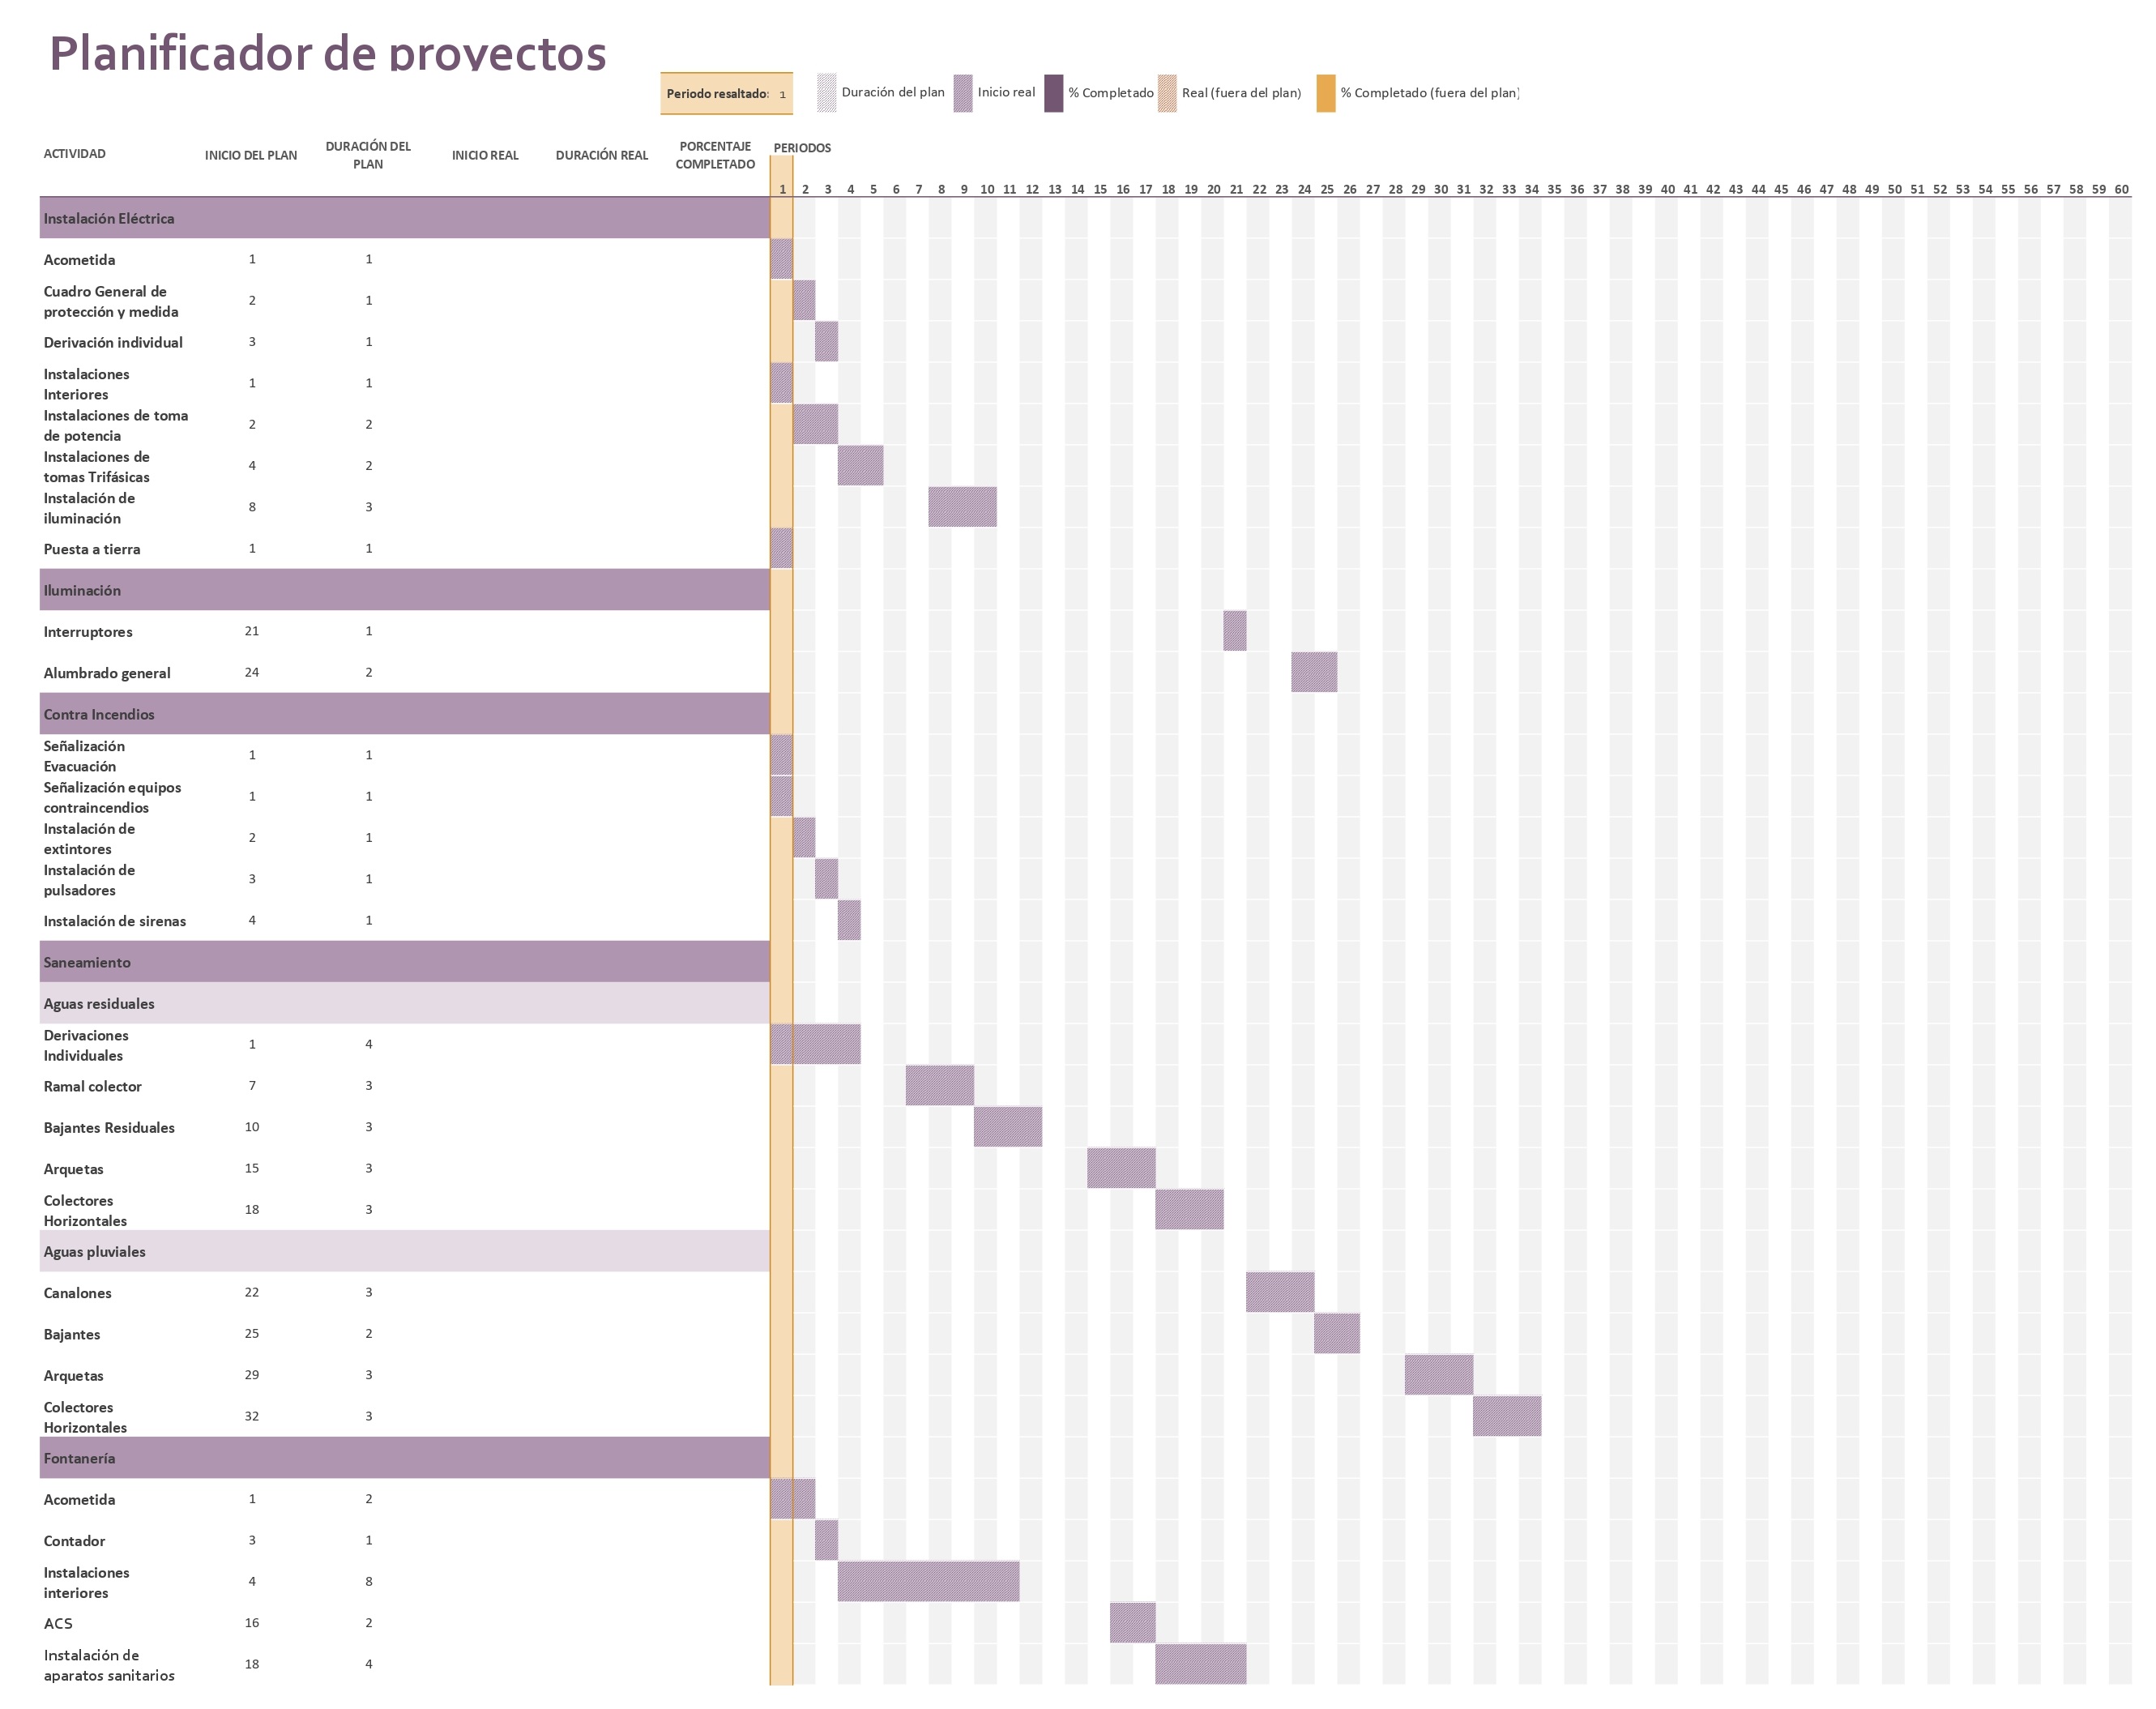
\includegraphics[width=1\linewidth]{Imagenes/Planificacion.png}
    \caption{Organización de las tareas y organigrama gantt.}
\end{figure}

\section{Orden de prioridad entre los documentos básicos}
% En este capítulo de la Memoria el autor del Proyecto, frente a posibles discrepancias, deberá estableces el orden de prioridad de los documentos básicos del Proyecto. Si no se especifica, el orden de prioridad será el siguiente: Planos - Pliego de Condiciones - Presupuesto - Memoria
Según la norma UNE 157001:2014, que establece los criterios generales para la elaboración formal de documentos de un proyecto técnico, se define el siguiente orden de prioridad para los documentos en este proyecto:
\begin{enumerate}
    \item Planos
    \item Pliego de condiciones
    \item Presupuestos
    \item Memoria
\end{enumerate}

\toftagstop{Memoria}
\end{document}